\documentclass[journal]{IEEEtran}

\usepackage[T1]{fontenc}
\usepackage[utf8]{inputenc}
\usepackage{cite}
\usepackage{amsmath,amssymb}
\usepackage{graphicx}
\usepackage{booktabs}
\usepackage{multirow}
\usepackage{xcolor}
\usepackage{microtype}
\usepackage[hidelinks]{hyperref}
\usepackage[capitalise,nameinlink]{cleveref}
\crefname{figure}{Fig.}{Figs.}
\crefname{table}{Table}{Tables}
\crefname{section}{Section}{Sections}

\graphicspath{{../figures/en/}}
% Généré par src/08_paper_assets.py — ne pas modifier à la main.
\newcommand{\resAAAAucA}{0.733}
\newcommand{\resAucAbsAFifty}{0.869}
\newcommand{\resAucAbsATen}{0.735}
\newcommand{\resAucAbsATwentyFive}{0.800}
\newcommand{\resAucAbsBFifty}{0.857}
\newcommand{\resAucAbsBTen}{0.720}
\newcommand{\resAucAbsBTwentyFive}{0.787}
\newcommand{\resAucRelAFifty}{0.878}
\newcommand{\resAucRelATen}{0.749}
\newcommand{\resAucRelATwentyFive}{0.816}
\newcommand{\resAucRelBFifty}{0.871}
\newcommand{\resAucRelBTen}{0.740}
\newcommand{\resAucRelBTwentyFive}{0.809}
\newcommand{\resBBBCost}{0.046}
\newcommand{\resBBBDrift}{+0.19}
\newcommand{\resConcAbs}{0.60}
\newcommand{\resConcGGGAbs}{0.79}
\newcommand{\resConcGGGRel}{0.70}
\newcommand{\resConcRel}{0.82}
\newcommand{\resCostAbs}{0.013}
\newcommand{\resCostRel}{0.008}
\newcommand{\resDriftAbs}{0.137}
\newcommand{\resDriftRecalK}{0.058}
\newcommand{\resDriftRecalT}{0.096}
\newcommand{\resDriftRel}{0.021}
\newcommand{\resFoneAbsATwentyFive}{0.653}
\newcommand{\resFoneAbsBTwentyFive}{0.638}
\newcommand{\resFoneRawK}{0.639}
\newcommand{\resFoneRecalK}{0.647}
\newcommand{\resFoneRelATwentyFive}{0.667}
\newcommand{\resFoneRelBTwentyFive}{0.661}
\newcommand{\resFprGenderAbsA}{$-$0.007}
\newcommand{\resFprGenderAbsACI}{[$-$0.019, +0.005]}
\newcommand{\resFprGenderAbsB}{+0.188}
\newcommand{\resFprGenderAbsBCI}{[+0.174, +0.201]}
\newcommand{\resFprGenderRelB}{+0.016}
\newcommand{\resFprGenderRelBCI}{[+0.004, +0.027]}
\newcommand{\resFprGenderWithinMax}{$-$0.023}
\newcommand{\resFprImdAbsA}{+0.148}
\newcommand{\resFprImdAbsB}{+0.163}
\newcommand{\resFprImdRelB}{+0.113}
\newcommand{\resFprImdRelChange}{$-$0.051}
\newcommand{\resFprImdRelChangeCI}{[$-$0.075, $-$0.026]}
\newcommand{\resGGGAucA}{0.739}
\newcommand{\resGGGClickPctile}{11}
\newcommand{\resGGGDrift}{+0.51}
\newcommand{\resGGGDriftFifty}{+0.52}
\newcommand{\resGGGDriftRecalK}{$-$0.04}
\newcommand{\resGGGDriftRel}{$-$0.01}
\newcommand{\resGGGDriftThirtyThree}{+0.60}
\newcommand{\resGGGFlagA}{44}
\newcommand{\resGGGFlagB}{95}
\newcommand{\resGGGMedClicks}{81}
\newcommand{\resGGGMedScore}{69}
\newcommand{\resGGGNoScore}{47}
\newcommand{\resGGGPrecA}{0.55}
\newcommand{\resGGGPrecB}{0.38}
\newcommand{\resGGGPrecRecalK}{0.55}
\newcommand{\resGGGPrecRecalT}{0.49}
\newcommand{\resGGGRecA}{0.66}
\newcommand{\resGGGRecB}{0.99}
\newcommand{\resGGGRecRecalT}{0.75}
\newcommand{\resGGGRisk}{37}
\newcommand{\resGGGShapDemo}{$-$0.02}
\newcommand{\resGGGShapEngage}{+0.12}
\newcommand{\resGGGShapScores}{+0.19}
\newcommand{\resGGGShapTotal}{+0.30}
\newcommand{\resGGGShapTotalRel}{$-$0.04}
\newcommand{\resGapAbsMax}{0.015}
\newcommand{\resGapAbsMin}{0.011}
\newcommand{\resGapRelMax}{0.009}
\newcommand{\resGapRelMin}{0.006}
\newcommand{\resGoneMax}{28.0}
\newcommand{\resGoneMaxMod}{CCC}
\newcommand{\resGoneMin}{5.4}
\newcommand{\resGoneMinMod}{GGG}
\newcommand{\resNActive}{26,232}
\newcommand{\resNConcImproved}{6}
\newcommand{\resNCorrTests}{69}
\newcommand{\resNEnrol}{32,593}
\newcommand{\resNGoneBeforeStart}{2,678}
\newcommand{\resNModules}{7}
\newcommand{\resNPres}{22}
\newcommand{\resOthersMedClicks}{432}
\newcommand{\resOthersMedScore}{79}
\newcommand{\resPctGone}{19.5}
\newcommand{\resPctLateSub}{4.0}
\newcommand{\resPctWithdrawnGone}{62.5}
\newcommand{\resPooledActiveA}{0.815}
\newcommand{\resPooledGap}{0.027}
\newcommand{\resPrecAbsATwentyFive}{0.669}
\newcommand{\resPrecAbsBTwentyFive}{0.617}
\newcommand{\resPrecRelATwentyFive}{0.697}
\newcommand{\resPrecRelBTwentyFive}{0.684}
\newcommand{\resRecAbsATwentyFive}{0.649}
\newcommand{\resRecAbsBTwentyFive}{0.722}
\newcommand{\resRecRelATwentyFive}{0.648}
\newcommand{\resRecRelBTwentyFive}{0.652}
\newcommand{\resRefA}{0.882}
\newcommand{\resRefB}{0.848}
\newcommand{\resRefGap}{0.033}
\newcommand{\resRhoAgeDifficulty}{$-$0.96}
\newcommand{\resRhoAgeDifficultyPres}{$-$0.79}
\newcommand{\resRhoShapDrift}{0.68}
\newcommand{\resRhoWithdrawnDrift}{$-$0.71}
\newcommand{\resRiskActive}{41.4}
\newcommand{\resRiskAll}{52.8}
\newcommand{\resRiskLowClicksGGG}{47}
\newcommand{\resRiskLowClicksOthers}{79}
\newcommand{\resRiskNoScoreGGG}{51}
\newcommand{\resRiskNoScoreOthers}{98}
\newcommand{\resRiskQFive}{33}
\newcommand{\resRiskQOne}{51}
\newcommand{\resSameAggGap}{0.013}
\newcommand{\resShareFemaleBBB}{88}
\newcommand{\resShareFemaleGGG}{81}
\newcommand{\resStabAbs}{0.81}
\newcommand{\resStabRel}{0.81}
\newcommand{\resTopFiveAbs}{3.3}
\newcommand{\resTopFiveRel}{4.0}
\newcommand{\resWdAucAAbs}{0.651}
\newcommand{\resWdAucARel}{0.675}
\newcommand{\resWdAucBAbs}{0.630}
\newcommand{\resWdAucBRel}{0.668}
\newcommand{\resWdCostAbs}{0.021}
\newcommand{\resWdCostRel}{0.006}
\newcommand{\resWdDriftAbs}{0.052}
\newcommand{\resWdDriftRel}{0.028}
\newcommand{\resWdGGGDriftAbs}{+0.18}
\newcommand{\resWdGGGDriftRel}{+0.03}
\newcommand{\resWdRecBAbs}{0.13}
\newcommand{\resWdRecBRel}{0.10}
\newcommand{\resWdRisk}{13.7}


\newcommand{\cA}{(A)}
\newcommand{\cB}{(B)}

\begin{document}

\title{The Ranking Transfers, the Threshold Does Not:\\ Early Dropout Prediction in Unseen Course Contexts}

% TODO (auteurs) : confirmer la liste et l'ordre des auteurs, et l'adresse de correspondance.
\author{Doudou~Coly and El~Hadji~Mamadou~Nguer%
\thanks{D. Coly and E. H. M. Nguer are with the Universit\'e Num\'erique Cheikh Hamidou Kane (UN-CHK), Dakar, Senegal.}}

\markboth{Preprint}{Coly and Nguer: The Ranking Transfers, the Threshold Does Not}

\maketitle

\begin{abstract}
Early-warning systems for online higher education are usually trained and evaluated within a single institution, on random splits that place the same courses in training and test sets, and often with features computed over the whole course. Before such a system is deployed in a new programme or institution, two questions must be answered: how much predictive signal is available early in a course, and what survives the move to a course the model has never seen? We study both on the Open University Learning Analytics Dataset (OULAD; \resNEnrol{} enrolments, \resNModules{} modules), using only data from the first 10--50\% of each presentation and a leave-one-module-out (LOMO) protocol. An audit of the evaluation pipeline first shows that three common choices---keeping students who have already withdrawn at the prediction date, using scores submitted after it, and comparing a pooled AUC with a per-module average---more than double the apparent transfer gap (\resRefGap{} versus \resSameAggGap{}). We then separate ranking from thresholding. Ranking transfers almost entirely (mean AUC cost \resCostAbs{} at 25\% of the course), but the decision threshold does not: in one module the share of flagged students rises from \resGGGFlagA\% to \resGGGFlagB\% for an observed risk of \resGGGRisk\%. Signed SHAP attributions show that the transferred model uses the same features as local models but reads them on absolute scales---engagement volumes, formative scores---whose meaning depends on course design. Re-expressing engagement and early scores as within-cohort percentile ranks, which needs no labels and is available at prediction time, cuts the mean flag-rate drift from \resDriftAbs{} to \resDriftRel{} and raises LOMO AUC from \resAucAbsBTwentyFive{} to \resAucRelBTwentyFive{}, outperforming Platt recalibration on 100 labelled students. The same drift appears with gradient boosting and a recurrent network, and models using weekly activity sequences gain at most \resGruGainMax{} AUC over the forest. Finally, threshold drift turns into group disparity through course composition: a female--male false-positive gap of \resFprGenderAbsB{} appears under LOMO although no module shows one internally; relative features remove it.
\end{abstract}

\begin{IEEEkeywords}
Learning analytics, dropout prediction, early warning systems, transferability, dataset shift, calibration, SHAP, algorithmic fairness, OULAD.
\end{IEEEkeywords}

%=====================================================================
\section{Introduction}
\label{sec:intro}

\IEEEPARstart{D}{ropout} remains one of the main obstacles to the promise of online higher education. Learning management systems (LMS) record student activity from the first day of a course, which has made data-driven early-warning systems an attractive way to target support while there is still time to act. The Open University Learning Analytics Dataset (OULAD) \cite{kuzilek2017oulad} has become the reference benchmark for this task: it is open, large, and combines demographics, registration, virtual learning environment (VLE) clickstreams and assessments for 22 module presentations. A recent systematic review counts a steady stream of predictive studies built on it \cite{jin2024slr}.

High accuracy on OULAD is no longer informative in itself. Two limitations recur in the recent literature and both matter when a model is to be used elsewhere. First, many studies compute predictors over the whole presentation; a 2026 regional fairness audit notes that its design is retrospective and that several of its predictors span the whole presentation \cite{elsayed2026fairness}. Such models cannot inform intervention, which must happen early. Second, models are almost always evaluated inside one institution, on splits that keep the same courses on both sides. A 2026 study predicting learner outcomes from the first 25\% of each presentation names its single-institution scope as a limit to external generalization \cite{malkani2026kronecker}; a calibrated early-warning study on OULAD splits by course presentation, so other presentations of a test module can still appear in training \cite{wu2026calibrated}. Outside OULAD, the evidence that predictive models are course-specific is strong \cite{gasevic2016onesize,conijn2017lms,lopezzambrano2020portability}, yet the mechanism of the failure is rarely examined.

This gap is concrete for institutions that would deploy an early-warning system without a labelled history of their own, such as the authors' fully online university in Senegal, where the target courses differ from any training course in design, assessment calendar and population. The relevant question is not whether a model achieves a high AUC on held-out students of known courses, but what part of its behaviour survives the move to a course it has never seen, why, and what can be done before labels exist.

We address this question on OULAD with an evaluation that is honest about timing and context. Predictions use only data available at a cut-off day placed at 10--50\% of each presentation, and we compare a random split grouped by student, protocol \cA, with leave-one-module-out, protocol \cB, in which each module plays the role of an unseen context. Our contributions are:
\begin{enumerate}
\item \emph{A methodological audit.} We show that three choices common in OULAD pipelines inflate early performance and the apparent transfer gap: keeping students already withdrawn at the cut-off (\resPctGone\% of enrolments at 25\%), using scores submitted after the cut-off, and comparing a pooled AUC in \cA{} with a per-module mean in \cB. Corrected, the transfer gap falls from \resRefGap{} to \resSameAggGap{} (\cref{tab:audit}).
\item \emph{A decomposition of transfer.} We separate intrinsic module difficulty, the transfer cost on ranking, and the drift of the decision threshold. Ranking transfers almost entirely; the threshold does not, and the modules that look hardest are difficult rather than untransferable (\cref{sec:transfer}).
\item \emph{A mechanism.} Using a transferred-versus-local SHAP comparison and a decomposition of the drift into signed attributions, we show that the transferred model relies on the same features as local ones but reads them on absolute scales whose meaning depends on course design. Global $|$SHAP$|$ importance cannot reveal this (\cref{sec:shap}).
\item \emph{A label-free remedy.} Re-expressing engagement and early scores as percentile ranks within the cohort removes the threshold drift and improves ranking, and compares favourably with Platt recalibration on small labelled samples (\cref{sec:remedies}).
\item \emph{A fairness consequence.} We show that threshold drift across contexts converts into a gender disparity through course composition, an effect that pooled fairness audits read as discrimination and within-context audits do not (\cref{sec:fairness}).
\item \emph{Independence from the learner.} Gradient boosting and a recurrent network on weekly activity sequences reproduce the same drift and the same correction, and the temporal signal adds little to early prediction (\cref{sec:sequence}).
\end{enumerate}

%=====================================================================
\section{Related Work}
\label{sec:related}

\subsection{Early prediction on OULAD}
OULAD was released to support the at-risk prediction work of the Open University \cite{kuzilek2017oulad}. Studies have since varied the observation window, for instance predicting at several percentages of the course length \cite{adnan2021percentages}, or from the first 25\% of each presentation with deep architectures \cite{malkani2026kronecker}. Wu et~al.\ \cite{wu2026calibrated} use a 28-day window, calibrate a gradient-boosting model, and audit subgroup fairness and alert capacity; their split holds out course presentations, not modules. Hlosta et~al.\ \cite{hlosta2017ouroboros} address a related cold-start problem at the Open University by training on the running presentation itself rather than on legacy data. We complement these studies by holding out entire modules and by asking which parts of the model's behaviour survive.

\subsection{Portability of predictive models across courses}
The Open Academic Analytics Initiative showed that a model trained at one institution could be ported to others with moderate loss \cite{jayaprakash2014oaai}. Course-level analyses are less optimistic: Ga\v{s}evi\'c et~al.\ \cite{gasevic2016onesize} found that the predictive value of LMS indicators depends on instructional conditions, Conijn et~al.\ \cite{conijn2017lms} that models varied substantially across 17 courses of a single institution, and L\'opez-Zambrano et~al.\ \cite{lopezzambrano2020portability} that direct transfer between Moodle courses works only under some conditions. Riestra-Gonz\'alez et~al.\ \cite{riestra2021massive} built course-agnostic early predictors from massive LMS logs, and Boyer and Veeramachaneni \cite{boyer2015transfer} studied transfer learning across MOOC offerings. These works measure whether accuracy transfers; we decompose \emph{what} fails to transfer and why.

\subsection{Dataset shift and calibration}
A change of context is a case of dataset shift, in which covariate, prior or concept changes can affect a classifier \cite{morenotorres2012shift}. In clinical prediction, it is well established that discrimination often survives a change of setting while calibration does not, and that simple updating of the intercept or slope on local data restores much of it \cite{janssen2008updating,vancalster2019calibration}. Platt scaling \cite{platt1999probabilistic} is the corresponding tool for machine-learning classifiers. Learning analytics has paid less attention to calibration under transfer, although decisions to contact students are taken at a threshold.

\subsection{Fairness of predictive student models}
Fairness audits of student models compare error rates and alert rates across demographic groups \cite{gardner2019slicing,baker2022bias}. On OULAD, recent studies document accuracy--fairness trade-offs \cite{opoku2025tradeoffs}, regional disparities in recall \cite{elsayed2026fairness} and policy-dependent alert-rate gaps \cite{wu2026calibrated}. When base rates differ between groups, error-rate parity and calibration cannot all hold \cite{chouldechova2017fair,kleinberg2017tradeoffs}; equal opportunity \cite{hardt2016equality} focuses on true-positive rates. We add a structural observation: aggregating over contexts can create group disparities that exist in no context, an instance of Simpson's paradox \cite{simpson1951}.

%=====================================================================
\section{Data and Methods}
\label{sec:methods}

\subsection{Dataset and target}
OULAD \cite{kuzilek2017oulad} (CC-BY 4.0) contains \resNEnrol{} enrolments in \resNPres{} presentations of \resNModules{} modules (AAA--GGG) at the Open University, UK. Each enrolment has a final result among Distinction, Pass, Fail and Withdrawn. Our main target is $y=1$ for Withdrawn or Fail (\resRiskAll\% of enrolments), since both outcomes call for the same early support; \cref{sec:robustness} repeats the analyses with Withdrawn only.

\subsection{Early window, population and features}
For a presentation $p$ of length $L_p$ days, the cut-off day is $d_c=\mathrm{round}(c\,L_p)$ with $c\in\{0.10,0.20,0.25,0.33,0.50\}$; $c=0.25$ is the reference. The population at $d_c$ consists of the students registered on or before $d_c$ and not unregistered by $d_c$. Students who have already left cannot be helped by an early warning, and keeping them makes the task artificially easy (\cref{sec:audit}).

For each enrolment we compute eighteen predictors from data dated on or before $d_c$:
\emph{demographics} (gender, region, highest education, IMD band, age band, previous attempts, studied credits, disability);
\emph{registration} (registration date relative to the course start and days registered in advance);
\emph{VLE engagement} (total clicks, active days, distinct resources, first and last active day, clicks per active day);
\emph{early assessments} (number of assessments, and mean score of those, whose deadline \emph{and} submission both fall on or before $d_c$). Missing engagement is coded as zero activity, missing first and last active days by out-of-range sentinels, and a missing early score as $-1$.

\paragraph*{Leakage control} Beyond excluding the final result and the unregistration date from the predictors \cite{kaufman2012leakage}, we test the whole pipeline by invariance: removing every raw record dated after $d_c$ (clicks, submissions, deadlines, unregistrations) must leave the feature table unchanged. The test detects, for instance, a filter on assessment deadlines alone, which lets late submissions through (\resPctLateSub\% of the retained submissions at $c=0.25$).

\subsection{Absolute and context-relative features}
The \emph{absolute} feature set uses the values above, as is usual. The \emph{relative} set replaces the eight engagement and early-assessment features by their percentile rank within the presentation,
\begin{equation}
\tilde{x}_{ij} = \frac{1}{n_p}\Big(L_{ij} + \frac{E_{ij}+1}{2}\Big),
\label{eq:rank}
\end{equation}
where $P_p$ is the population of presentation $p$ at $d_c$, $n_p=|P_p|$, $L_{ij}$ counts the students of $P_p$ whose value of feature $j$ is lower than $x_{ij}$, and $E_{ij}$ those, $i$ included, whose value equals it (average rank for ties). Demographic and registration features are unchanged. The transformation uses no labels and only data available at the cut-off, and it passes the invariance test.

\subsection{Model and protocols}
We use a random forest \cite{breiman2001rf} of 300 trees with balanced class weights (scikit-learn \cite{pedregosa2011sklearn}, one-hot encoding of categorical variables, seed 0) and flag a student when the predicted probability $\hat{p}\geq 0.5$. Protocol \cA{} is a five-fold split stratified on $y$ and grouped by student, so that no student appears in both training and test folds; its out-of-fold predictions cover every enrolment. Protocol \cB{} trains on six modules and predicts the seventh, for each module in turn.

Both protocols are summarized in the same way: metrics are computed on the students of each module, then averaged over modules. An AUC pooled over all modules in \cA{} would reward the model for separating modules with different base rates, which \cB{} cannot do by construction.

For each module $m$ we define three quantities on the same students:
\begin{align}
\text{difficulty:}\quad & D_m = \mathrm{AUC}_{A}(m), \\
\text{ranking cost:}\quad & C_m = \mathrm{AUC}_{A}(m) - \mathrm{AUC}_{B}(m), \\
\text{flag-rate drift:}\quad & \Delta_m = \bar{f}_{B}(m) - \bar{f}_{A}(m),
\end{align}
where $\bar{f}(m)$ is the share of the module's students flagged. $D_m$ measures how predictable a module is when the model has seen it, $C_m$ how much ranking is lost when it has not, and $\Delta_m$ how far the volume of alerts moves.

\subsection{Sequential features and alternative learners}
\label{sec:seqmethods}
To test whether temporal information or another learner changes the picture, we build weekly sequences over the $K$ complete weeks observed before the cut-off in \emph{every} presentation, $K=\lfloor(\min_p d_c+1)/7\rfloor$ (3, 6, 8, 11 and 16 weeks for the five cut-offs), so that all sequences have the same length and use only data dated on or before $d_c$. Each week has two channels, clicks and active days; we add pre-course clicks and four trend features (slope of $\log(1+\text{clicks})$ over the weeks, share of clicks in the second half of the window, number of active weeks, weeks since the last active one). In the relative variant these columns are also ranked within the presentation. They pass the invariance test.

We compare the random forest with three models: histogram gradient boosting (scikit-learn, balanced class weights) on the aggregated features, the same with the sequences and trends added, and a gated recurrent unit (GRU) network. The GRU reads the two-channel weekly sequence (hidden size 32); a dense layer encodes the static features (aggregated features, trends, demographics); both are concatenated before a logistic output. It is trained with Adam (learning rate $2\times10^{-3}$, batches of 256, at most 30 epochs) on a loss weighted by the inverse class frequencies, so that the 0.5 threshold has the same meaning as for the forest, with early stopping on a stratified 10\% split of the training data. All models are evaluated with protocols \cA{} and \cB{} as above.

\subsection{Remedies}
We compare two ways of correcting the transferred model. \emph{Platt recalibration} \cite{platt1999probabilistic} fits a logistic regression of $y$ on $\mathrm{logit}(\hat{p}_B)$, with balanced weights as in the source model, on labelled students of the target module: either $k\in\{25,50,100,200\}$ students drawn at random (50 draws, evaluation on the remaining students), or the first presentation of the module as a pilot cohort, evaluated on later presentations. \emph{Relative features} (\cref{eq:rank}) require no labels.

\subsection{Context descriptors}
To explain heterogeneity, each module and presentation is described by its assessment structure (number of assessments due before the cut-off, first non-exam deadline as a fraction of the presentation, share of the exam in the total weight), observable engagement (share of students with an early score, median clicks, number of VLE activity types) and population (size, at-risk rate, share of Withdrawn among at-risk students, share without A-levels, share aged 35 or more), plus the standardized distance of the assessment structure to that of the other modules. We report Spearman correlations with $D_m$, $C_m$ and $\Delta_m$ at the module level ($n=7$) and the presentation level ($n=22$; presentations of a module share its LOMO model and are not independent), with Benjamini--Hochberg control of the false discovery rate within level \cite{benjamini1995fdr}.

\subsection{Interpretability}
We compute SHAP values \cite{lundberg2017shap} with TreeSHAP \cite{lundberg2020treeshap} for two models per module $m$: the \emph{transferred} LOMO model, and a \emph{local} model trained on $m$ alone with two-fold cross-fitting grouped by student (each half is explained by the model trained on the other). Attributions of one-hot columns are summed back to their original variable. Exact TreeSHAP on unpruned forests is slow (about 1.7\,s per student for 300 trees); since the SHAP value of a forest is the average of those of its trees, we estimate it without bias from 100 trees drawn at random, which reproduces the exact importance ranking with Spearman $\rho=0.985$. We explain 400 students per module.

Two analyses follow. The \emph{agreement} between transferred and local models is the Spearman correlation of their global importances (mean $|\phi|$) over the 18 variables. The \emph{drift decomposition} averages signed attributions of the transferred model over the students of $m$ and over feature families $G$:
\begin{equation}
\bar{\phi}_{m,G} = \frac{1}{|S_m|}\sum_{i\in S_m}\sum_{j\in G}\phi_{ij}.
\label{eq:decomp}
\end{equation}
By local accuracy, the sum over all families equals the mean difference between the predicted risk of $m$'s students and the average prediction on the training modules.

\subsection{Fairness}
We compare true-positive rate (TPR), false-positive rate (FPR), precision (PPV) and flag rate between women and men, the most and least deprived IMD quintiles (Q1: 0--20\%; Q5: 80--100\%), and students with and without a declared disability. Confidence intervals (95\%) come from a cluster bootstrap over students with 1{,}000 resamples \cite{efron1993bootstrap}; the same resamples are used for all configurations, which gives paired intervals for changes in gaps.

\subsection{Implementation and reproducibility}
All analyses run in Python 3.12 with scikit-learn 1.9.1, pandas 3.0.6, shap 0.54.1 and PyTorch 2.14.1 (CPU), with fixed seeds. A single script regenerates every figure, table and number of this article from the raw OULAD files, and an automated test suite checks the absence of leakage.
% TODO (code) : ajouter l'URL du dépôt public au moment de la soumission.

%=====================================================================
\section{Results}
\label{sec:results}

\begin{table}[t]
\centering
\caption{Methodological audit at the 25\% cut-off (random forest). Each row adds one correction to the previous one. AUC of protocol (A), random split grouped by student, and (B), leave-one-module-out (LOMO), mean over held-out modules.}
\label{tab:audit}
\begin{tabular}{@{}p{4.3cm}ccc@{}}
\toprule
Evaluation setting & AUC (A) & AUC (B) & Gap \\
\midrule
1) Reference protocol (all enrolments, pooled AUC in (A)) & 0.882 & 0.848 & 0.033 \\
2) + early scores filtered on submission date & 0.880 & 0.849 & 0.031 \\
3) + students still enrolled at the cut-off only & 0.815 & 0.787 & 0.027 \\
4) + same aggregation in (A) and (B) & 0.800 & 0.787 & 0.013 \\
5) + context-relative features & 0.816 & 0.809 & 0.008 \\
\bottomrule
\end{tabular}
\end{table}


\subsection{Methodological audit}
\label{sec:audit}
The reference pipeline we started from, which keeps all enrolments and compares a pooled AUC in \cA{} with a per-module mean in \cB, gives AUC \resRefA{} in \cA{} and \resRefB{} in \cB{} at 25\% of the course, a transfer gap of \resRefGap{} (\cref{tab:audit}). Filtering early scores on their submission date changes little. Restricting the population to students still enrolled at the cut-off has the largest effect: at 25\%, \resPctGone\% of enrolments have already ended, \resPctWithdrawnGone\% of all Withdrawn outcomes among them, including \resNGoneBeforeStart{} unregistrations before the course started. Their last active day makes them trivial to predict, and their share ranges from \resGoneMin\% (\resGoneMinMod) to \resGoneMax\% (\resGoneMaxMod), which confounds any comparison between modules. Finally, comparing like with like halves the gap again, from \resPooledGap{} to \resSameAggGap. Together, these choices make the apparent transfer gap more than twice its corrected value. Context-relative features reduce it further to \resCostRel.

\subsection{How early can we predict?}
\cref{fig:early} shows performance against the length of the observed window. With relative features, AUC rises from \resAucRelATen{} at 10\% of the course to \resAucRelAFifty{} at 50\% in \cA, and from \resAucRelBTen{} to \resAucRelBFifty{} in \cB; the gap between protocols stays between \resGapRelMin{} and \resGapRelMax{} at every cut-off (\resGapAbsMin--\resGapAbsMax{} with absolute features). With absolute features, the transferred model flags too many students: at 25\%, its recall exceeds that of \cA{} (\resRecAbsBTwentyFive{} versus \resRecAbsATwentyFive) while its precision falls (\resPrecAbsBTwentyFive{} versus \resPrecAbsATwentyFive). With relative features, recall and precision of \cB{} track those of \cA{} (\resRecRelBTwentyFive{} versus \resRecRelATwentyFive; \resPrecRelBTwentyFive{} versus \resPrecRelATwentyFive). Reporting recall alone, a common practice for at-risk prediction, would have made the transferred model look better than the local one.

\begin{figure*}[t]
\centering
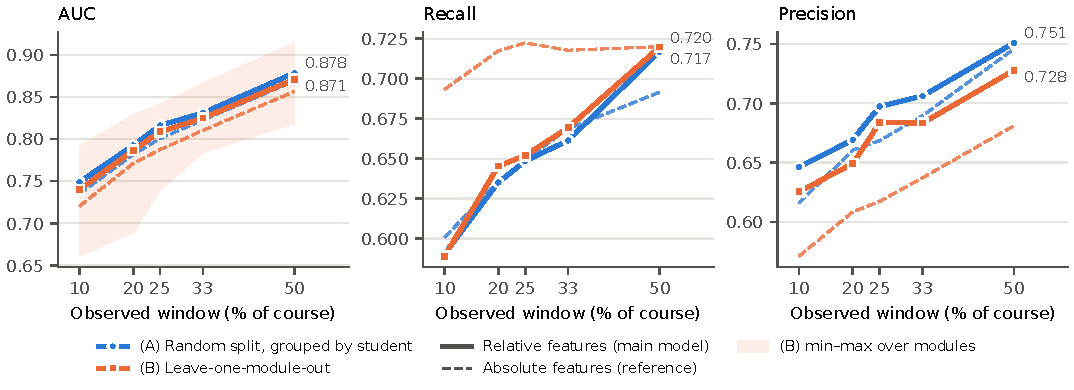
\includegraphics[width=\textwidth]{early_curve}
\caption{Performance against the observed share of the presentation (students still enrolled at the cut-off). Solid lines: relative features; dashed lines: absolute features. Both protocols are averaged over modules in the same way; the band shows the range over held-out modules in \cB{} with relative features.}
\label{fig:early}
\end{figure*}

\begin{table*}[t]
\centering
\caption{Module characteristics at the 25\% cut-off, students still enrolled at the cut-off. At-risk: Withdrawn or Fail. First deadline: first non-exam assessment, as a fraction of the presentation length. Exam weight: share of the exam in the total assessment weight. Early score: share of students with at least one assessment submitted before the cut-off. Values are averaged over the presentations of each module.}
\label{tab:modules}
\footnotesize
\begin{tabular}{@{}lrrrrrrrr@{}}
\toprule
 & & At-risk & Withdrawn among & First & Exam & Early & Median & Aged \\
Module & $n$ & (\%) & at-risk (\%) & deadline & weight (\%) & score (\%) & clicks & 35+ (\%) \\
\midrule
AAA & 698 & 23.9 & 45.5 & 0.07 & 50 & 98.1 & 588 & 52.6 \\
BBB & 6,202 & 39.5 & 28.0 & 0.07 & 50 & 93.4 & 224 & 34.9 \\
CCC & 3,191 & 47.4 & 48.4 & 0.07 & 67 & 93.1 & 402 & 30.3 \\
DDD & 4,984 & 47.7 & 40.7 & 0.09 & 50 & 93.4 & 382 & 26.2 \\
EEE & 2,470 & 33.2 & 31.6 & 0.13 & 50 & 90.9 & 586 & 24.9 \\
FFF & 6,289 & 42.0 & 35.4 & 0.08 & 50 & 94.5 & 866 & 26.2 \\
GGG & 2,398 & 36.9 & 17.6 & 0.24 & 100 & 53.3 & 81 & 39.0 \\
\bottomrule
\end{tabular}
\end{table*}


\subsection{The ranking transfers, the threshold does not}
\label{sec:transfer}
\cref{tab:transfer} and \cref{fig:transfer} separate the three quantities per module at 25\%. The ranking cost is small: \resCostAbs{} on average with absolute features, and below 0.015 for six modules out of seven; BBB is the exception (\resBBBCost). Modules AAA and GGG, which a naive reading of LOMO results would call ``poorly transferable'', are in fact \emph{difficult}: their AUC is already low when the model has seen them (\resAAAAucA{} and \resGGGAucA{}), and it drops by only 0.013 when it has not.

The threshold is another matter. In GGG, the transferred model flags \resGGGFlagB\% of students, against \resGGGFlagA\% for the model that has seen the module and an observed risk of \resGGGRisk\%: recall climbs from \resGGGRecA{} to \resGGGRecB{} and precision falls from \resGGGPrecA{} to \resGGGPrecB. BBB drifts too (\resBBBDrift), CCC and DDD slightly downwards. The mean absolute drift is \resDriftAbs. An institution that deployed such a model in a GGG-like course would contact almost every student.

\begin{table*}[t]
\centering
\caption{Ranking versus threshold transfer per module (25\% cut-off, students still enrolled). AUC and flag rate ($p \geq 0.5$) are computed on the students of each module; (A) uses out-of-fold predictions of the random split, (B) the model trained on the six other modules.}
\label{tab:transfer}
\begin{tabular}{@{}lccccccccc@{}}
\toprule
 & \multicolumn{3}{c}{Ranking (absolute features)} & \multicolumn{3}{c}{Flagged students, \% (absolute)} & \multicolumn{2}{c}{Relative features, (B)} \\
\cmidrule(lr){2-4}\cmidrule(lr){5-7}\cmidrule(l){8-9}
Module & AUC (A) & AUC (B) & Cost & Observed risk & (A) & (B) & AUC & Flagged (\%) \\
\midrule
AAA & 0.733 & 0.720 & +0.013 & 24 & 35 & 44 & 0.793 & 37 \\
BBB & 0.796 & 0.750 & +0.046 & 39 & 37 & 56 & 0.804 & 40 \\
CCC & 0.830 & 0.825 & +0.004 & 47 & 44 & 40 & 0.813 & 45 \\
DDD & 0.837 & 0.830 & +0.007 & 48 & 44 & 39 & 0.842 & 39 \\
EEE & 0.841 & 0.844 & $-$0.004 & 33 & 26 & 33 & 0.838 & 30 \\
FFF & 0.828 & 0.816 & +0.012 & 42 & 36 & 34 & 0.833 & 36 \\
GGG & 0.739 & 0.726 & +0.013 & 37 & 44 & 95 & 0.739 & 30 \\
\midrule
Mean & 0.800 & 0.787 & +0.013 & 39 & 38 & 49 & 0.809 & 37 \\
\bottomrule
\end{tabular}
\end{table*}


\begin{figure*}[t]
\centering
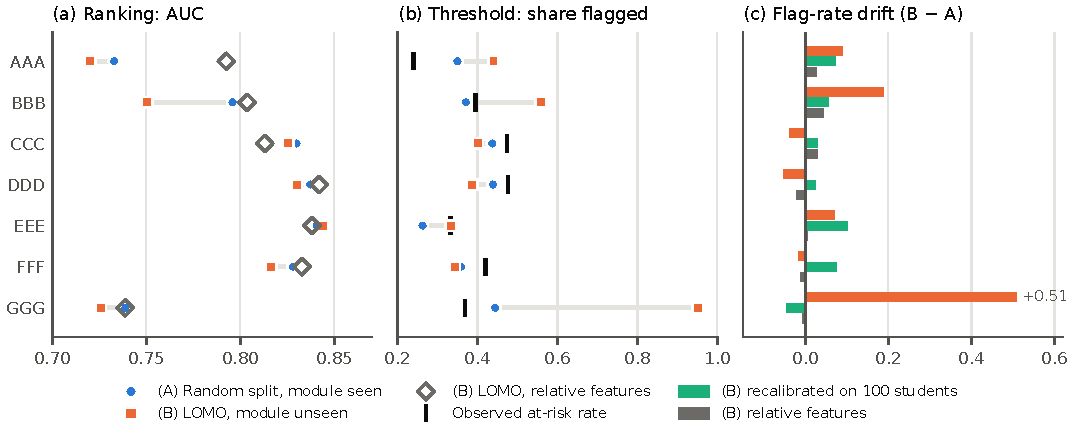
\includegraphics[width=\textwidth]{transfer}
\caption{Ranking versus threshold per module at the 25\% cut-off. (a) AUC when the module is seen \cA{} or unseen \cB, and \cB{} with relative features. (b) Share of students flagged in \cA{} and \cB{} against the observed at-risk rate. (c) Flag-rate drift of the raw transferred model, after Platt recalibration on 100 labelled students of the module, and with relative features.}
\label{fig:transfer}
\end{figure*}

\subsection{Why GGG drifts}
\label{sec:mechanism}
\cref{tab:modules} shows how GGG differs from the other modules. Its first non-exam assessment falls at about a quarter of the presentation instead of 7--13\%, its assignments are formative (the exam carries the whole weight), and only half of its students have an early score at the cut-off. Its students also use the VLE much less: their median click count before the cut-off is \resGGGMedClicks{} against \resOthersMedClicks{} in the other modules, the \resGGGClickPctile{}th percentile of the latter. Elsewhere, students with at most \resGGGMedClicks{} clicks are at risk in \resRiskLowClicksOthers\% of cases; in GGG, \resRiskLowClicksGGG\%. Elsewhere, a student without an early score is at risk in \resRiskNoScoreOthers\% of cases; in GGG, where \resGGGNoScore\% of students have none yet, \resRiskNoScoreGGG\%. Early scores are also lower (median \resGGGMedScore{} against \resOthersMedScore{}). The drift is not limited to the period before the first deadline: it reaches \resGGGDriftThirtyThree{} at 33\% and \resGGGDriftFifty{} at 50\% of the course.

In short, the model has learned absolute thresholds---``few clicks'' or ``no score yet'' means risk---whose meaning depends on the design of the course. \cref{tab:corr} gives the associations that survive multiple-testing control. Difficulty is associated with the share of older students (Spearman $\rho$~=~\resRhoAgeDifficulty{} over modules, \resRhoAgeDifficultyPres{} over presentations). Drift is larger where at-risk students fail rather than withdraw ($\rho$~=~\resRhoWithdrawnDrift), where students are older and less qualified, and where the VLE is used less. The structural distance of the assessment design to the other modules is associated with drift, not with the ranking cost, which is weakly associated with an earlier and denser assessment calendar. With seven modules, these associations are exploratory; the experiments below test the mechanism directly.

\begin{table}[t]
\centering
\caption{Context descriptors associated with the three transfer axes (Spearman's $\rho$, Benjamini--Hochberg $q < 0.10$ within level, 69 tests in total). Mod.: modules; Pres.: presentations, which are not independent (they share the module-level LOMO model). Difficulty: AUC (A); Rank.\ cost: AUC (A) $-$ AUC (B); Drift: flag-rate drift. Exploratory associations.}
\label{tab:corr}
\footnotesize
\begin{tabular}{@{}llp{3.3cm}rr@{}}
\toprule
Level ($n$) & Axis & Descriptor & $\rho$ & $q$ \\
\midrule
Mod. (7) & Difficulty & Share aged 35+ & $-$0.96 & 0.016 \\
Pres. (22) & Difficulty & Share aged 35+ & $-$0.79 & 0.000 \\
Pres. (22) & Difficulty & VLE activity types & +0.54 & 0.037 \\
Pres. (22) & Difficulty & At-risk rate & +0.49 & 0.060 \\
Pres. (22) & Rank. cost & First deadline & $-$0.55 & 0.037 \\
Pres. (22) & Rank. cost & Share with early score & +0.52 & 0.042 \\
Pres. (22) & Rank. cost & Assessments due before cut-off & +0.46 & 0.078 \\
Pres. (22) & Drift & Withdrawn share among at-risk & $-$0.71 & 0.004 \\
Pres. (22) & Drift & Share aged 35+ & +0.62 & 0.023 \\
Pres. (22) & Drift & At-risk rate & $-$0.61 & 0.023 \\
Pres. (22) & Drift & Share without A-level & +0.58 & 0.029 \\
Pres. (22) & Drift & Median clicks & $-$0.57 & 0.029 \\
Pres. (22) & Drift & Assessment-structure distance & +0.53 & 0.042 \\
Pres. (22) & Drift & VLE activity types & $-$0.48 & 0.063 \\
Pres. (22) & Drift & Assessments due before cut-off & $-$0.45 & 0.082 \\
\bottomrule
\end{tabular}
\end{table}


\subsection{Interpretability: same features, wrong thresholds}
\label{sec:shap}
If transfer failed because different features matter in different modules, global importances would differ between transferred and local models. They mostly do not. Local models rank the 18 variables similarly across modules (mean pairwise Spearman \resStabAbs), with the mean early score first everywhere. Agreement between transferred and local importances is moderate with absolute features (mean \resConcAbs, \resTopFiveAbs{} of the top five variables in common) and higher with relative features (\resConcRel, \resTopFiveRel{} in common), an improvement in \resNConcImproved{} modules out of seven (\cref{fig:shap}a). Crucially, GGG---the module that drifts most---shows one of the \emph{highest} agreements with absolute features (\resConcGGGAbs). Its problem is not which features are used but how they are read.

The drift decomposition of \cref{eq:decomp} makes this visible (\cref{fig:shap}b). On GGG's students, the transferred absolute model raises predicted risk by \resGGGShapTotal{} above its training average: \resGGGShapScores{} from early-score features and \resGGGShapEngage{} from engagement, while demographics contribute \resGGGShapDemo. Across modules, this total follows the flag-rate drift ($\rho$~=~\resRhoShapDrift). With relative features the decomposition vanishes (\resGGGShapTotalRel{} for GGG; \cref{fig:shap}c). Global importance, which discards the sign of attributions, cannot detect a threshold problem; signed attributions on the target population can.

\begin{figure*}[t]
\centering
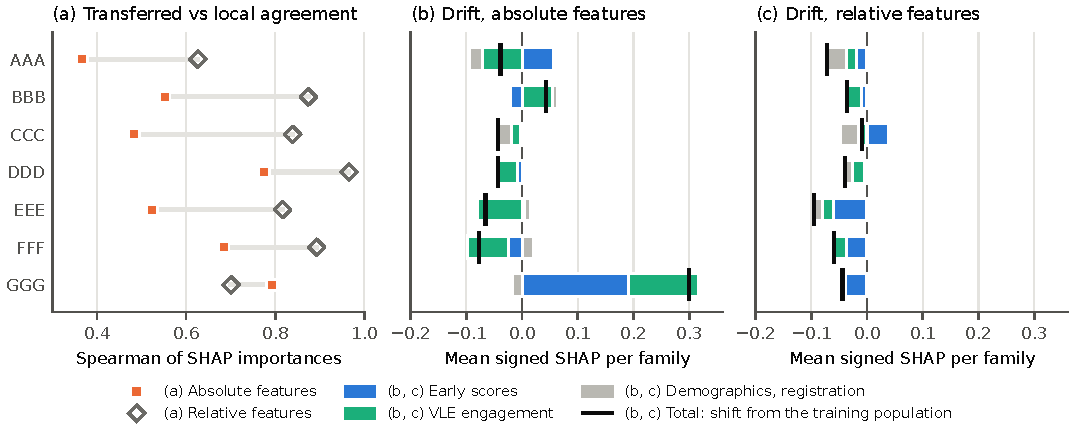
\includegraphics[width=\textwidth]{shap}
\caption{Same features, wrong thresholds (25\% cut-off). (a) Spearman correlation between the SHAP importances of the transferred model and of a model trained on the module itself. (b, c) Mean signed SHAP attribution of the transferred model on the students of each module, by feature family: the shift of their predicted risk from the training population.}
\label{fig:shap}
\end{figure*}

\subsection{Remedies}
\label{sec:remedies}
\cref{tab:remedies} compares the two corrections. Platt recalibration on 100 labelled students of the target module reduces the mean absolute drift from \resDriftAbs{} to \resDriftRecalK{} and repairs GGG (drift \resGGGDriftRecalK, precision \resGGGPrecB{}~$\rightarrow$~\resGGGPrecRecalK). Using the first presentation as a pilot cohort is less effective on average (\resDriftRecalT), because presentations of the same module also differ; it still helps GGG (precision \resGGGPrecRecalT, recall \resGGGRecRecalT{} instead of \resGGGRecB). Recalibration leaves the ranking unchanged and moves F1 little (\resFoneRawK{} to \resFoneRecalK{} on average), since F1 rewards over-flagging when risk is common.

Relative features do better without any label: mean absolute drift \resDriftRel, GGG drift \resGGGDriftRel, and an AUC of \resAucRelBTwentyFive{} on unseen modules---higher than that of the absolute model on modules it has seen (\resAucAbsATwentyFive). Mean precision and F1 of \cB{} rise to \resPrecRelBTwentyFive{} and \resFoneRelBTwentyFive. The ranks discard information on the absolute level of engagement in a cohort, but this information was precisely what did not transfer.

\begin{table*}[t]
\centering
\caption{Flag-rate drift (B) $-$ (A) and precision of the transferred model under the two remedies (25\% cut-off). Platt-$k$: Platt recalibration on $k=100$ randomly drawn labelled students of the target module (mean of 50 draws, evaluated on the remaining students). Platt-pilot: recalibration on the first presentation of the module, evaluated on the later ones (drift measured against (A) on the same students). Relative: context-relative features, no labels.}
\label{tab:remedies}
\begin{tabular}{@{}lcccccccc@{}}
\toprule
 & \multicolumn{4}{c}{Flag-rate drift} & \multicolumn{4}{c}{Precision of (B)} \\
\cmidrule(lr){2-5}\cmidrule(l){6-9}
Module & Raw & Platt-$k$ & Platt-pilot & Relative & Raw & Platt-$k$ & Platt-pilot & Relative \\
\midrule
AAA & +0.09 & +0.07 & +0.09 & +0.03 & 0.38 & 0.38 & 0.38 & 0.46 \\
BBB & +0.19 & +0.06 & +0.15 & +0.04 & 0.54 & 0.60 & 0.53 & 0.67 \\
CCC & $-$0.04 & +0.03 & $-$0.11 & +0.03 & 0.78 & 0.74 & 0.85 & 0.73 \\
DDD & $-$0.05 & +0.03 & +0.04 & $-$0.02 & 0.79 & 0.75 & 0.73 & 0.81 \\
EEE & +0.07 & +0.10 & +0.14 & +0.01 & 0.69 & 0.66 & 0.62 & 0.72 \\
FFF & $-$0.02 & +0.08 & +0.07 & $-$0.01 & 0.76 & 0.69 & 0.70 & 0.76 \\
GGG & +0.51 & $-$0.04 & +0.08 & $-$0.01 & 0.38 & 0.55 & 0.49 & 0.64 \\
\midrule
Mean $|\cdot|$ / mean & 0.14 & 0.06 & 0.10 & 0.02 & 0.62 & 0.62 & 0.61 & 0.68 \\
\bottomrule
\end{tabular}
\end{table*}


\subsection{Fairness}
\label{sec:fairness}
\cref{tab:fairness} and \cref{fig:fairness} report error-rate gaps between groups. With absolute features, transfer creates a gender gap that does not exist when modules are seen: the FPR gap between women and men moves from \resFprGenderAbsA{} \resFprGenderAbsACI{} in \cA{} to \resFprGenderAbsB{} \resFprGenderAbsBCI{} in \cB. Yet inside every module the transferred model's FPR is \emph{lower} for women (the largest within-module gap is \resFprGenderWithinMax; \cref{fig:fairness}c). The pooled gap is a composition effect: women make up \resShareFemaleBBB\% of BBB and \resShareFemaleGGG\% of GGG, the two modules whose threshold drifts upwards, so the drift of these modules is attributed to gender when modules are pooled \cite{simpson1951}. With relative features, the gap falls to \resFprGenderRelB{} \resFprGenderRelBCI.

IMD and disability gaps behave differently. They exist under every protocol and reflect different base rates (\resRiskQOne\% at risk in Q1 against \resRiskQFive\% in Q5): the most deprived students are flagged more often, correctly and incorrectly (FPR gap \resFprImdAbsA{} in \cA, \resFprImdAbsB{} in \cB). Relative features reduce the FPR gap in \cB{} by \resFprImdRelChange{} \resFprImdRelChangeCI{} without closing it, consistent with the impossibility of equalizing error rates and calibration when base rates differ \cite{chouldechova2017fair,kleinberg2017tradeoffs}.

\begin{table*}[t]
\centering
\caption{Between-group gaps in error rates at the 25\% cut-off (threshold 0.5), with 95\% confidence intervals from a student-level cluster bootstrap (1{,}000 resamples). TPR: recall; FPR: false-positive rate; PPV: precision; Flag: share of students flagged.}
\label{tab:fairness}
\footnotesize
\setlength{\tabcolsep}{4pt}
\begin{tabular}{@{}llcccc@{}}
\toprule
Contrast & Configuration & TPR gap & FPR gap & PPV gap & Flag-rate gap \\
\midrule
\multirow{3}{*}{Female $-$ male} & (A) absolute & $-$0.080 [$-$0.096, $-$0.061] & $-$0.007 [$-$0.019, +0.005] & $-$0.042 [$-$0.058, $-$0.025] & $-$0.050 [$-$0.062, $-$0.038] \\
 & (B) absolute & +0.014 [$-$0.003, +0.031] & +0.188 [+0.174, +0.201] & $-$0.168 [$-$0.184, $-$0.151] & +0.105 [+0.093, +0.117] \\
 & (B) relative & $-$0.062 [$-$0.080, $-$0.044] & +0.016 [+0.004, +0.027] & $-$0.061 [$-$0.077, $-$0.043] & $-$0.029 [$-$0.042, $-$0.018] \\
\midrule
\multirow{3}{*}{IMD Q1 $-$ Q5} & (A) absolute & +0.135 [+0.104, +0.165] & +0.148 [+0.127, +0.169] & +0.044 [+0.013, +0.077] & +0.224 [+0.205, +0.243] \\
 & (B) absolute & +0.143 [+0.113, +0.173] & +0.163 [+0.139, +0.189] & +0.102 [+0.073, +0.133] & +0.223 [+0.203, +0.245] \\
 & (B) relative & +0.125 [+0.092, +0.157] & +0.113 [+0.092, +0.133] & +0.062 [+0.032, +0.095] & +0.203 [+0.182, +0.224] \\
\midrule
\multirow{3}{*}{Disability yes $-$ no} & (A) absolute & +0.095 [+0.067, +0.121] & +0.102 [+0.076, +0.128] & +0.020 [$-$0.006, +0.047] & +0.146 [+0.124, +0.167] \\
 & (B) absolute & +0.060 [+0.034, +0.085] & +0.098 [+0.069, +0.126] & +0.047 [+0.022, +0.076] & +0.119 [+0.097, +0.140] \\
 & (B) relative & +0.080 [+0.052, +0.107] & +0.064 [+0.039, +0.090] & +0.041 [+0.015, +0.068] & +0.120 [+0.097, +0.141] \\
\bottomrule
\end{tabular}
\end{table*}


\begin{figure*}[t]
\centering
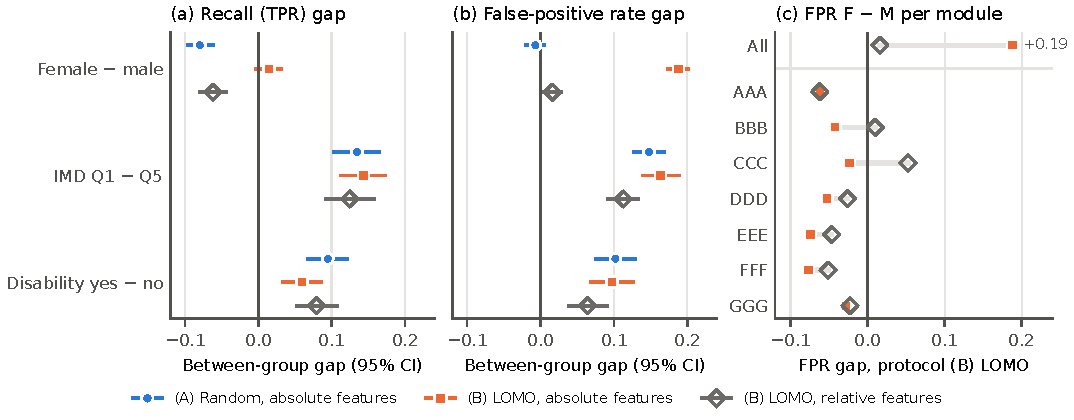
\includegraphics[width=\textwidth]{fairness}
\caption{Error-rate gaps between groups (25\% cut-off, 95\% cluster-bootstrap intervals). (a) Recall and (b) false-positive rate gaps. (c) Female--male FPR gap of the transferred model computed inside each module and over all modules: the pooled gap of the absolute model is a composition effect.}
\label{fig:fairness}
\end{figure*}

\subsection{Sequences and other learners}
\label{sec:sequence}
\cref{tab:sequence} and \cref{fig:sequence} repeat the analysis with gradient boosting and the GRU. Temporal information adds little to early prediction: on unseen modules with relative features, adding weekly sequences and trends to gradient boosting raises AUC by at most \resSeqGainMax{} across cut-offs, and the GRU exceeds the forest by \resGruGainMin{} to \resGruGainMax. At these windows, the aggregated counts already carry most of the early signal.

The threshold problem, in contrast, does not depend on the learner. With absolute features, all four models drift by \resDriftAbsModelsMin{} to \resDriftAbsModelsMax{} on average at 25\%, and GGG by \resGGGDriftModelsMin{} to \resGGGDriftModelsMax. Relative features reduce the drift for every model, to \resDriftRelGru{} for the GRU, which also has the smallest ranking cost (\resCostGruRel), and to \resDriftRelHgb{} for gradient boosting, whose residual drift is spread over modules with alternating signs rather than concentrated in one design. The mechanism identified with the forest is a property of the features, not of the learner.

\begin{table}[t]
\centering
\caption{Model families and temporal information at the 25\% cut-off (students still enrolled; means over modules). Forest and Boosting: aggregated features; Boosting + seq.: aggregated features plus weekly clicks and active days over the complete weeks before the cut-off and trend features; GRU: recurrent network on the weekly sequence plus all static features. Cost: AUC (A) $-$ AUC (B); Drift: mean absolute flag-rate drift; GGG: drift in module GGG.}
\label{tab:sequence}
\footnotesize
\setlength{\tabcolsep}{3pt}
\begin{tabular}{@{}llccccc@{}}
\toprule
Features & Model & AUC (A) & AUC (B) & Cost & Drift & GGG \\
\midrule
\multirow{4}{*}{Absolute} & Forest & 0.800 & 0.787 & +0.013 & 0.137 & +0.51 \\
 & Boosting & 0.805 & 0.789 & +0.016 & 0.132 & +0.53 \\
 & Boosting + seq. & 0.808 & 0.794 & +0.014 & 0.128 & +0.52 \\
 & GRU & 0.799 & 0.793 & +0.006 & 0.118 & +0.47 \\
\midrule
\multirow{4}{*}{Relative} & Forest & 0.816 & 0.809 & +0.008 & 0.021 & $-$0.01 \\
 & Boosting & 0.818 & 0.811 & +0.007 & 0.055 & +0.01 \\
 & Boosting + seq. & 0.819 & 0.812 & +0.007 & 0.055 & +0.00 \\
 & GRU & 0.817 & 0.815 & +0.002 & 0.031 & +0.02 \\
\bottomrule
\end{tabular}
\end{table}


\begin{figure*}[t]
\centering
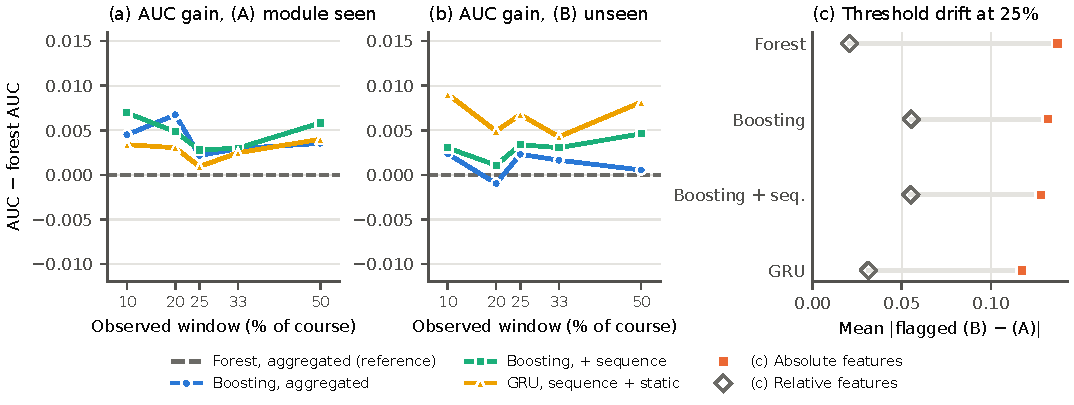
\includegraphics[width=\textwidth]{sequence}
\caption{Sequences and other learners (students still enrolled). (a, b) AUC gain over the aggregated random forest (dashed zero line) with relative features, when the module is seen \cA{} or unseen \cB. (c) Mean absolute flag-rate drift at the 25\% cut-off with absolute and relative features.}
\label{fig:sequence}
\end{figure*}

\subsection{Robustness to the target definition}
\label{sec:robustness}
Restricted to students still enrolled at the cut-off, ``Withdrawn only'' becomes \emph{future} withdrawal, a rarer (\resWdRisk\% at 25\%) and harder target (\cref{tab:target}). At the 0.5 threshold, the balanced forest rarely flags such students (recall \resWdRecBAbs{} in \cB), so we compare on AUC. The pattern holds: relative features lower the ranking cost from \resWdCostAbs{} to \resWdCostRel{}, the mean absolute drift from \resWdDriftAbs{} to \resWdDriftRel{} (GGG: \resWdGGGDriftAbs{} to \resWdGGGDriftRel), and raise LOMO AUC from \resWdAucBAbs{} to \resWdAucBRel.

\begin{table}[t]
\centering
\caption{Robustness to the target definition (25\% cut-off, students still enrolled; means over modules). W or F: Withdrawn or Fail; W only: Withdrawn only. Abs./rel.: absolute or relative features. Cost: AUC (A) $-$ AUC (B); Drift: mean absolute flag-rate drift.}
\label{tab:target}
\footnotesize
\setlength{\tabcolsep}{3pt}
\begin{tabular}{@{}llcccccc@{}}
\toprule
Target & Feat. & Risk (\%) & AUC (A) & AUC (B) & Cost & Drift & GGG \\
\midrule
W or F & abs. & 38.7 & 0.800 & 0.787 & +0.013 & 0.137 & +0.51 \\
W or F & rel. & 38.7 & 0.816 & 0.809 & +0.008 & 0.021 & $-$0.01 \\
W only & abs. & 13.7 & 0.651 & 0.630 & +0.021 & 0.052 & +0.18 \\
W only & rel. & 13.7 & 0.675 & 0.668 & +0.006 & 0.028 & +0.03 \\
\bottomrule
\end{tabular}
\end{table}


%=====================================================================
\section{Discussion}
\label{sec:discussion}

\subsection{What transfers and what does not}
Our results draw a sharper picture of model portability than an accuracy gap. The ordering of students by risk is largely shared across modules: early scores, recent activity and the number of submissions predict risk everywhere, as local models confirm. What is specific to a course is the scale on which these signals are expressed: how many clicks a normal week requires, when the first assessment is due, whether early assignments are graded. A model that learns absolute thresholds carries the scale of its training courses into the new one. The parallel with clinical prediction models, where discrimination travels better than calibration \cite{janssen2008updating,vancalster2019calibration}, is close, and so are the remedies.

\subsection{Implications for deployment in a new context}
For an institution starting an early-warning system without labelled history, three practical recommendations follow. First, express engagement and early-assessment features relative to the cohort at the prediction date. This needs no outcome data, only a cohort observed up to the same day, which online programmes have. Second, monitor the alert volume against expectations from the first weeks: a flag rate far from the expected risk is a warning sign of threshold drift, not a sign of an at-risk cohort. Third, once a first cohort is labelled, recalibrate; around a hundred labelled students sufficed here. The same reasoning applies across countries, where VLE usage and assessment practices may differ more than between modules of one university.

\subsection{Implications for evaluation practice}
Four lessons generalize beyond OULAD. Early-prediction studies should restrict the population to students still enrolled at the prediction date and check leakage by invariance, not only by excluding outcome variables. Comparisons between protocols must use the same aggregation. Threshold-based metrics should be reported with the alert rate, since recall alone rewards over-flagging. Fairness audits that pool contexts should be complemented by within-context audits; otherwise a calibration problem can read as discrimination and, conversely, a real within-context bias can be masked by composition.

\subsection{Limitations}
The study uses one institution and seven modules; module-level correlations have little power, and presentation-level ones are not independent. The threshold is fixed at 0.5 with balanced class weights; capacity-based alerting, which flags a fixed share of students \cite{wu2026calibrated}, fixes the alert volume by construction but leaves the share to be set for each new course, which is precisely what is unknown there. Gradient boosting and a GRU confirm the mechanism, but our GRU is deliberately small and other sequence architectures or richer event streams might extract more temporal signal. SHAP values are estimated from a subsample of trees and 400 students per module. Relative ranks remove between-cohort differences in the level of engagement, so a model using them cannot detect a whole cohort that is collectively disengaged; in very small cohorts, ranks are also noisy. IMD gaps remain and call for policy choices on how alerts are used. Finally, the transfer we study is between modules of one university; transfer across institutions and countries, which motivates this work, remains to be tested.

\subsection{Future work}
We will replay the same protocol on Moodle data from a fully online Senegalese university, where the held-out context becomes a degree programme and then a country, and study whether relative features also stabilize transfer across institutions whose VLE usage differs more than between modules of one university.

%=====================================================================
\section{Conclusion}
\label{sec:conclusion}
Measured honestly---early, on students still enrolled, and with comparable aggregation---the cost of moving an at-risk model to an unseen course is small for ranking and large for thresholds. The threshold fails because engagement and early scores are read on absolute scales that depend on course design; the same features matter everywhere. Expressing them relative to the cohort removes the drift without labels, improves ranking on unseen courses, and removes a gender disparity created by pooling contexts. Early-warning systems meant to travel should be evaluated on unseen contexts, report alert rates alongside accuracy, and audit fairness within contexts.

\section*{Data and Code Availability}
OULAD is available under a CC-BY 4.0 licence from the Open University (\url{https://analyse.kmi.open.ac.uk/open_dataset}). The code that reproduces every figure, table and number of this article is available from the authors and will be released in a public repository upon publication.

\bibliographystyle{IEEEtran}
\bibliography{references}

\end{document}
